\chapter{教育发展}
\label{chapter:Education}

习近平总书记深刻指出:“教育、科技、人才是全面建设社会主义现代化国家的基础性、战略性支撑。”这句话为新时代我国教育与科技的协同发展提供了战略指导。

在科技创新浪潮席卷全球的当下,教育不仅肩负着培养创新型人才的重要使命,更是推动科技进步的关键力量。十四届全国人大三次会议进一步强调,教育要与科技创新深度融合,依托人工智能等前沿技术,实现个性化、精准化培养,使得教育更具个性化、智能化特点,同时也为人才培养提供了更为广阔的平台。

此外,科技创新在教育中的广泛应用,有望有效缩小区域间的教育差距,推动教育公平普及,为全面建设社会主义现代化国家奠定坚实基础。


\section{资金投入推动科技创新}

教育支出占 GDP 的比重是衡量一个国家对教育重视程度的重要指标,直接反映了政府对教育的战略规划,并对教育质量提升、人才培养水平产生深远影响,从而与科技创新能力和社会发展紧密相连。

基于世界银行集团《教育公共开支总额》数据集,本研究绘制了各国教育支出占GDP的百分比变化趋势”折线图(见图\ref{01各国教育支出占GDP的百分比变化趋势图})。该图直观展示了各国教育支出占 GDP 比重的变化轨迹,为分析各国教育投入动态和政策效果提供了有力依据。

\begin{figure}[H]
    \centering
    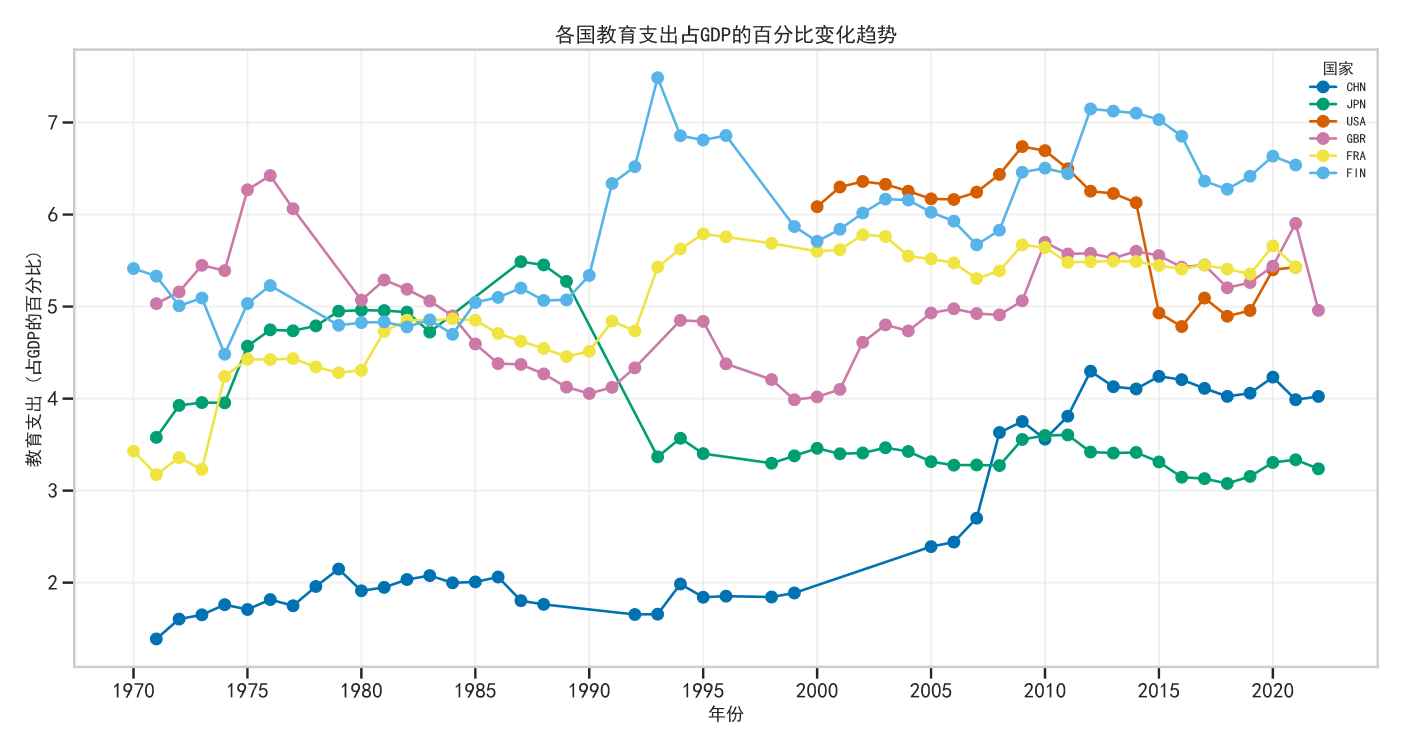
\includegraphics[width=0.7\linewidth]{figure/01各国教育支出占GDP的百分比变化趋势图.png}
    \caption{各国教育支出占GDP的百分比变化趋势图}
    \label{01各国教育支出占GDP的百分比变化趋势图}
\end{figure}

从图表中可以看出,中国的教育支出占GDP比例呈现明显上升趋势\cite{huang2021education},然而与其他国家相比仍有提升空间。具体来看,自2000年以来,中国的教育支出占比迅速攀升,尤其在2008年,即汶川地震后,出现了显著增长。这一现象可能归因于灾后学校重建、农村义务教育保障工程以及职业和高等教育的大规模扩招等多重因素共同作用。
\subsection{研究与试验发展经费支出趋势}
高等学校研究与试验发展(R\&D)经费支出的变化趋势,是衡量一国高等教育科研能力和创新投入的重要指标。基于国家统计局《高等学校科技活动情况》数据集,本研究绘制了“高等学校研究与试验发展经费支出变化趋势”折线图(见图\ref{fig:02高等学校研究与试验发展经费支出变化趋势图}),直观展示了各项经费投入随时间的变动情况。

\begin{figure}[H]
    \centering
    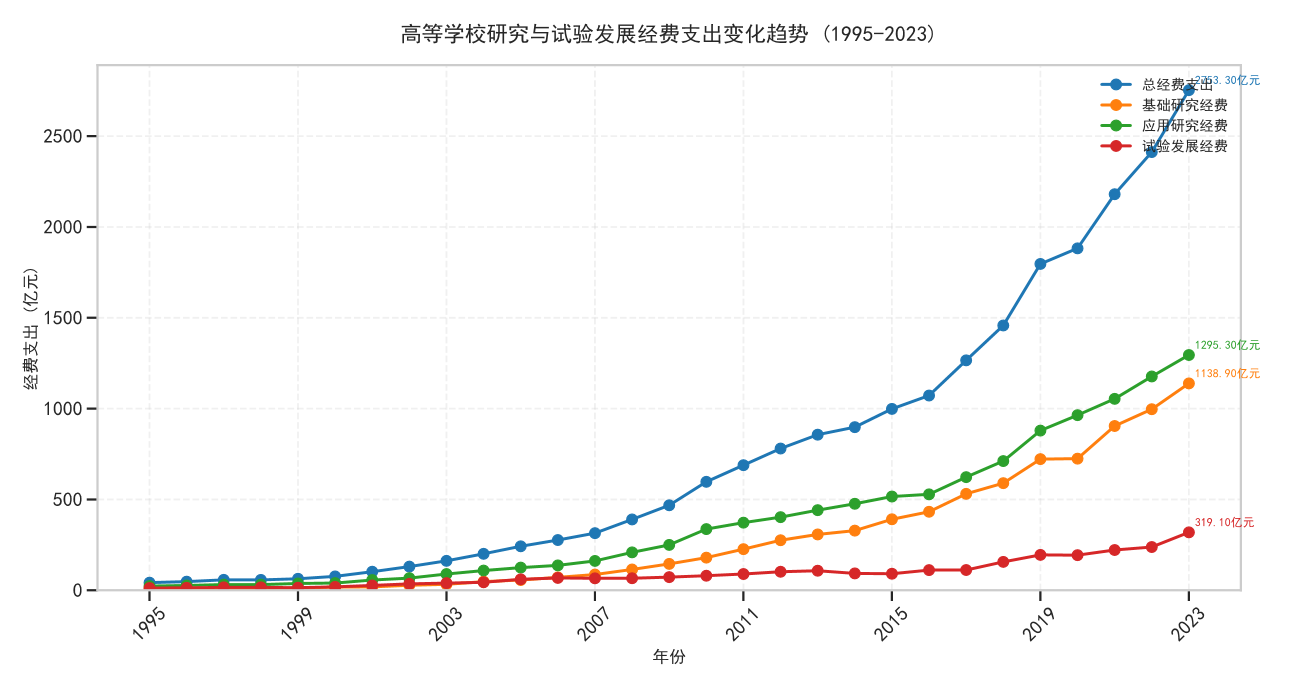
\includegraphics[width=0.8\linewidth]{figure/02高等学校研究与试验发展经费支出变化趋势图.png}
    \caption{高等学校研究与试验发展经费支出变化趋势图}
    \label{fig:02高等学校研究与试验发展经费支出变化趋势图}
\end{figure}

从图表中可以直观地看到,高等学校研究与试验发展经费的总支出呈现持续且大幅度增长的趋势\cite{Zhou2024},从1995年的不足百亿元增长至2023年的2500亿元以上。

分项经费方面,基础研究经费、应用研究经费和试验发展经费均显著增长,但其增速与占比有所差异。具体而言,试验研究经费在1995年时几乎可以忽略不计,但在2023年已达到319.1亿元;基础研究经费从较低基数逐步增长至1138.9亿元,显示出其在整体经费投入中所处的重要地位;应用研究经费的增长尤为突出,从最初的低水平跃升至1295.3亿元,稳居总经费支出的最大份额。

\subsection{研究与试验发展经费支出占比}
为更好地研究三大经费类别在整体投入中的比重变化,还绘制了“高等学校研究与试验发展经费支出占比变化”面积图(见图\ref{fig:03高等学校研究与试验发展经费支出占比变化})。

从面积图中可以看出,尽管试验发展经费的绝对数值不断攀升,但其在总体结构中的占比却出现了相对下降,这反映出当前高校在技术成果推广及实践转化方面可能存在一定的制约因素,需要进一步优化科研成果的转化机制和实践应用环节。

\begin{figure}[H]
    \centering
    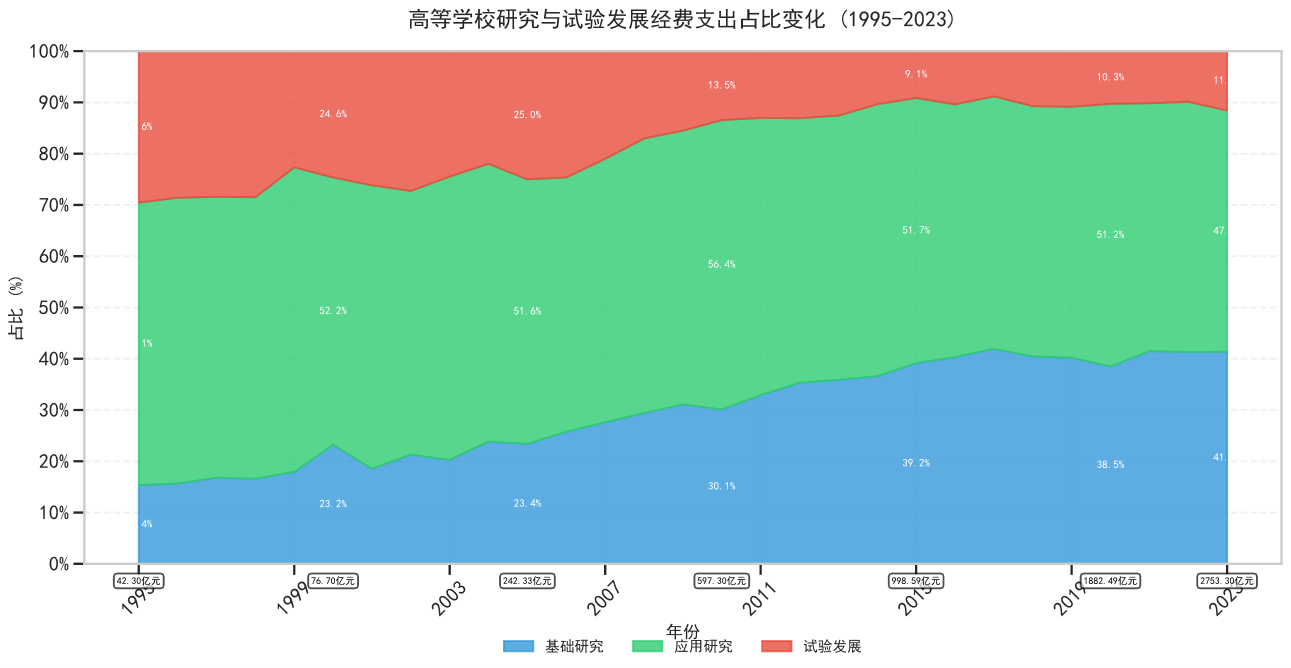
\includegraphics[width=0.7\linewidth]{figure/03高等学校研究与试验发展经费支出占比变化.png}
    \caption{高等学校研究与试验发展经费支出占比变化图}
    \label{fig:03高等学校研究与试验发展经费支出占比变化}
\end{figure}

这一现象表明,尽管高校科研经费整体快速增长,但在投入结构调控方面仍有优化空间。基础研究稳步上升显示出原始创新的重要性;而应用研究经费占比高,表明高校正加快成果转化。但试验发展经费尽管总额不断增加,其相对占比下降,暗示在科研成果实际应用和技术试验环节仍存在瓶颈,亟需完善相关政策机制。


\section{科技创新引领教育发展}

高校科研产出是衡量学术创新水平和科研能力的重要指标,其核心涵盖科研项目数量、科技论文数量以及专利授权数。基于国家统计局《高等学校科技活动情况》数据集,本研究绘制了“高校科研产出指标趋势对比与预测”折线图,并运用融合模型对未来趋势进行预测(见图\ref{fig:04高校科研产出指标趋势对比与预测图})。

\begin{figure}[H]
    \centering
    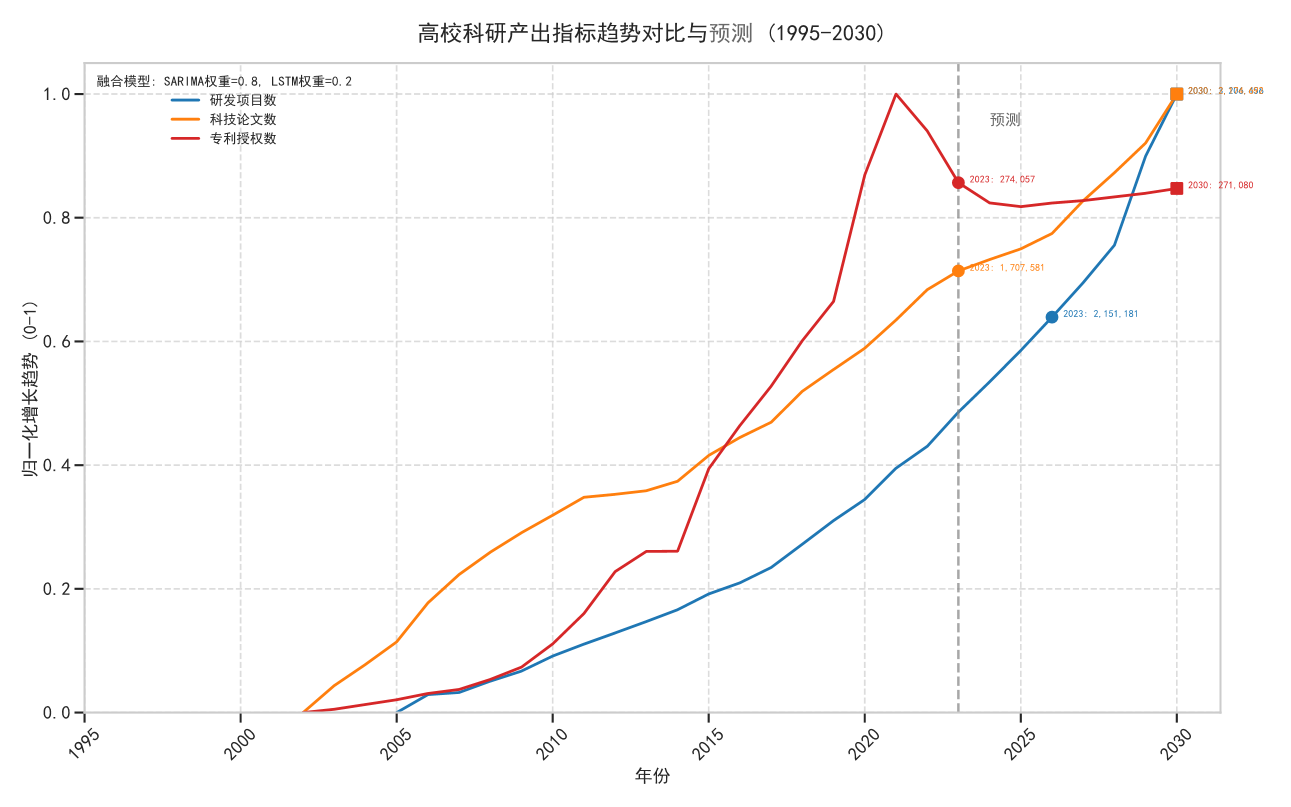
\includegraphics[width=0.7\linewidth]{figure/04高校科研产出指标趋势对比与预测图.png}
    \caption{高校科研产出指标趋势对比与预测图}
    \label{fig:04高校科研产出指标趋势对比与预测图}
\end{figure}

历史数据表明,科研项目数、科技论文数和专利授权数均显著增长,但各自阶段和增速不同。科研项目数自1995年稳步上升,至2023年达2,151,181,预计2030年将达3,206,458;科技论文数在2005–2015年间迅速攀升,至2023年达1,707,581,预计2030年将突破2,271,080;专利授权数虽波动较大(2020–2023年曾大幅下滑),但2010–2020年增速显著,2023年已达274,057,预计2030年将增至330,458。

近年来,中国政策逐步向质量导向转变,重点提升发明专利的审查标准,同时对实用新型和外观设计专利进行调整,2023年这两类专利分别下降了25.5\%和11.5\%。此外,“十四五”规划期间逐步取消专利补贴,可能进一步降低高校在低质量专利申请方面的积极性。

总体来看,科研项目数的稳步增长彰显了高校在科研投入和项目立项方面的提升;科技论文数的快速上升反映了学术影响力和国际合作的深化;而专利授权数的波动则既显示突破也暴露挑战。展望2030年,高校科研产出要在保持投入的同时,优化资源配置、加强国际合作、推动成果产业化,从而巩固其全球科技竞争地位.

\section{社会变革提供资金投入}
为探讨社会变革对未来科技创新的反作用,本研究基于前文对高校研究与试验发展经费未来五年走势的预测数据,绘制了“高等学校经费支出融合预测”折线图(见图\ref{fig:05高等学校研究与试验发展经费支出融合预测}),直观展示了未来经费支出的发展趋势。

\begin{figure}[H]
    \centering
    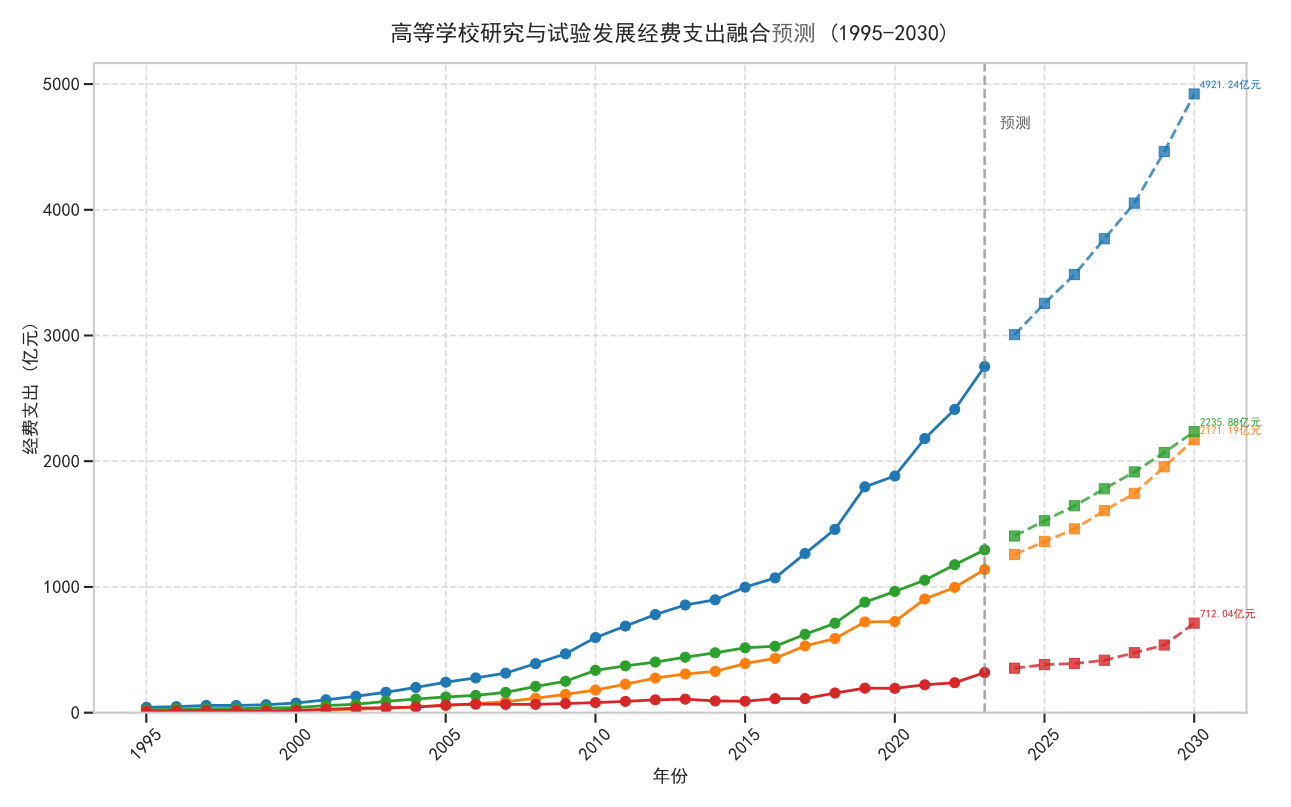
\includegraphics[width=0.7\linewidth]{figure/05高等学校研究与试验发展经费支出融合预测.png}
    \caption{高等学校研究与试验发展经费支出融合预测}
    \label{fig:05高等学校研究与试验发展经费支出融合预测}
\end{figure}

从实际数据来看,1995年至2023年间,高校科研总经费经历了指数级增长,从不足百亿元跃升至约3000亿元,预计到2030年将突破4900亿元。基础研究经费增长稳健,在极低基数的基础上迅速攀升至2023年的2171.19亿元,并预计2030年达到约2235.88亿元;应用研究经费亦持续稳步上升,2023年约为1500亿元,预测2030年将突破1700亿元。相比之下,试验发展经费虽然也呈现增长态势,但增速相对较小,2023年达到712.04亿元,预计2030年将接近800亿元。

具体的预测数据如表\ref{高校经费支出融合预测值(2024--2030)数据汇总}所示。

\begin{table}[H]
  \centering
  \caption{高校经费支出融合预测值(2024--2030)数据汇总表}
  \begin{minipage}[t]{0.48\textwidth}
    \centering
    \caption*{(a) 总经费支出预测(2024--2030)}
    \vspace{0.5em}
    \begin{tabular}{lc}
      \toprule
      年份 & 经费(亿元) \\
      \midrule
      2024 & 3006.26 \\
      2025 & 3255.37 \\
      2026 & 3484.90 \\
      2027 & 3769.74 \\
      2028 & 4052.68 \\
      2029 & 4463.49 \\
      2030 & 4921.24 \\
      \bottomrule
    \end{tabular}
  \end{minipage}
  \hfill
  \begin{minipage}[t]{0.48\textwidth}
    \centering
    \caption*{(b) 基础研究经费预测(2024--2030)}
    \vspace{0.5em}
    \begin{tabular}{lc}
      \toprule
      年份 & 经费(亿元) \\
      \midrule
      2024 & 1258.12 \\
      2025 & 1362.15 \\
      2026 & 1461.68 \\
      2027 & 1607.25 \\
      2028 & 1744.18 \\
      2029 & 1956.19 \\
      2030 & 2171.19 \\
      \bottomrule
    \end{tabular}
  \end{minipage}
  
  \vspace{1em}
  
  \begin{minipage}[t]{0.48\textwidth}
    \centering
    \caption*{(c) 应用研究经费预测(2024--2030)}
    \vspace{0.5em}
    \begin{tabular}{lc}
      \toprule
      年份 & 经费(亿元) \\
      \midrule
      2024 & 1405.42 \\
      2025 & 1526.58 \\
      2026 & 1645.90 \\
      2027 & 1781.00 \\
      2028 & 1914.91 \\
      2029 & 2068.88 \\
      2030 & 2235.88 \\
      \bottomrule
    \end{tabular}
  \end{minipage}
  \hfill
  \begin{minipage}[t]{0.48\textwidth}
    \centering
    \caption*{(d) 试验发展经费预测(2024--2030)}
    \vspace{0.5em}
    \begin{tabular}{lc}
      \toprule
      年份 & 经费(亿元) \\
      \midrule
      2024 & 353.74 \\
      2025 & 382.13 \\
      2026 & 391.36 \\
      2027 & 416.77 \\
      2028 & 476.90 \\
      2029 & 538.18 \\
      2030 & 712.04 \\
      \bottomrule
    \end{tabular}
  \end{minipage}
  
  \label{高校经费支出融合预测值(2024--2030)数据汇总}
\end{table}

高校科研经费的迅猛增长彰显了国家在科技创新领域持续加大投入,助推了高校科研能力的提升。基础研究经费以最快增速和显著占比增长,反映出高校在原始创新方面的加大投入,与国家对基础学科和前沿技术的重视相契合;应用研究经费的稳步上升突显了高校在解决实际问题和技术转化中的关键作用;而试验发展经费增长较缓,则表明技术应用和产业化领域仍需深化产学研合作。

总体来看,高校科研经费的逐年增长既验证了国家科技创新战略的成效,也凸显了高校在基础研究、应用研究和试验发展中的关键地位。未来,高校应在持续强化基础研究的同时,通过优化资源配置和深化产学研融合,提升科研质量和技术转化效率,从而在全球科技竞争中稳固并提升自身优势。
